\ifdefined\included
\else
\documentclass[a4paper,11pt,twoside]{StyleThese}
\usepackage{amsmath,amssymb}             % AMS Math
\usepackage[french]{babel}
\usepackage[utf8]{inputenc}
\usepackage[T1]{fontenc}
\usepackage{tabularx}
%\usepackage{tabular}
\usepackage{multirow}


\usepackage[tight,footnotesize]{subfigure}
\usepackage{algorithm} %To allow algorithm environment
\usepackage{algpseudocode} %Provides algorithmic environment

\usepackage{hhline}
\usepackage[left=1.5in,right=1.3in,top=1.1in,bottom=1.1in,includefoot,includehead,headheight=13.6pt]{geometry}
\renewcommand{\baselinestretch}{1.05}

% Table of contents for each chapter

\usepackage[nottoc, notlof, notlot]{tocbibind}
\usepackage[french]{minitoc}
\setcounter{minitocdepth}{2}
\mtcindent=15pt
% Use \minitoc where to put a table of contents

\usepackage{aecompl}

% Glossary / list of abbreviations

\usepackage[intoc]{nomencl}
\renewcommand{\nomname}{Liste des Abréviations}

\makenomenclature

% My pdf code

\usepackage{ifpdf}

\ifpdf
  \usepackage[pdftex]{graphicx}
  \DeclareGraphicsExtensions{.jpg}
  \usepackage[a4paper,pagebackref,hyperindex=true]{hyperref}
  \usepackage{tikz}
  \usetikzlibrary{arrows,shapes,calc}
\else
  \usepackage{graphicx}
  \DeclareGraphicsExtensions{.ps,.eps}
  \usepackage[a4paper,dvipdfm,pagebackref,hyperindex=true]{hyperref}
\fi

\graphicspath{{.}{images/}}

%nicer backref links
\renewcommand*{\backref}[1]{}
\renewcommand*{\backrefalt}[4]{%
\ifcase #1 %
(Non cité.)%
\or
(Cité en page~#2.)%
\else
(Cité en pages~#2.)%
\fi}
\renewcommand*{\backrefsep}{, }
\renewcommand*{\backreftwosep}{ et~}
\renewcommand*{\backreflastsep}{ et~}

% Links in pdf
\usepackage{color}
\definecolor{linkcol}{rgb}{0,0,0.4} 
\definecolor{citecol}{rgb}{0.5,0,0} 
\definecolor{linkcol}{rgb}{0,0,0} 
\definecolor{citecol}{rgb}{0,0,0}
% Change this to change the informations included in the pdf file

\hypersetup
{
bookmarksopen=true,
pdftitle="Évaluation de la sécurité des équipements grand public connectés à Internet",
pdfauthor="Yann BACHY", %auteur du document
pdfsubject="Thèse", %sujet du document
%pdftoolbar=false, %barre d'outils non visible
pdfmenubar=true, %barre de menu visible
pdfhighlight=/O, %effet d'un clic sur un lien hypertexte
colorlinks=true, %couleurs sur les liens hypertextes
pdfpagemode=None, %aucun mode de page
pdfpagelayout=SinglePage, %ouverture en simple page
pdffitwindow=true, %pages ouvertes entierement dans toute la fenetre
linkcolor=linkcol, %couleur des liens hypertextes internes
citecolor=citecol, %couleur des liens pour les citations
urlcolor=linkcol %couleur des liens pour les url
}

% definitions.
% -------------------

\setcounter{secnumdepth}{3}
\setcounter{tocdepth}{2}

% Some useful commands and shortcut for maths:  partial derivative and stuff

\newcommand{\pd}[2]{\frac{\partial #1}{\partial #2}}
\def\abs{\operatorname{abs}}
\def\argmax{\operatornamewithlimits{arg\,max}}
\def\argmin{\operatornamewithlimits{arg\,min}}
\def\diag{\operatorname{Diag}}
\newcommand{\eqRef}[1]{(\ref{#1})}

\usepackage{rotating}                    % Sideways of figures & tables
%\usepackage{bibunits}
%\usepackage[sectionbib]{chapterbib}          % Cross-reference package (Natural BiB)
%\usepackage{natbib}                  % Put References at the end of each chapter
                                         % Do not put 'sectionbib' option here.
                                         % Sectionbib option in 'natbib' will do.
\usepackage{fancyhdr}                    % Fancy Header and Footer

% \usepackage{txfonts}                     % Public Times New Roman text & math font
  
%%% Fancy Header %%%%%%%%%%%%%%%%%%%%%%%%%%%%%%%%%%%%%%%%%%%%%%%%%%%%%%%%%%%%%%%%%%
% Fancy Header Style Options

\pagestyle{fancy}                       % Sets fancy header and footer
\fancyfoot{}                            % Delete current footer settings

%\renewcommand{\chaptermark}[1]{         % Lower Case Chapter marker style
%  \markboth{\chaptername\ \thechapter.\ #1}}{}} %

%\renewcommand{\sectionmark}[1]{         % Lower case Section marker style
%  \markright{\thesection.\ #1}}         %

\fancyhead[LE,RO]{\bfseries\thepage}    % Page number (boldface) in left on even
% pages and right on odd pages
\fancyhead[RE]{\bfseries\nouppercase{\leftmark}}      % Chapter in the right on even pages
\fancyhead[LO]{\bfseries\nouppercase{\rightmark}}     % Section in the left on odd pages

\let\headruleORIG\headrule
\renewcommand{\headrule}{\color{black} \headruleORIG}
\renewcommand{\headrulewidth}{1.0pt}
\usepackage{colortbl}
\arrayrulecolor{black}

\fancypagestyle{plain}{
  \fancyhead{}
  \fancyfoot{}
  \renewcommand{\headrulewidth}{0pt}
}

%\usepackage{MyAlgorithm}
%\usepackage[noend]{MyAlgorithmic}
\usepackage[ED=MITT - STICIA, Ets=INP]{tlsflyleaf}
%%% Clear Header %%%%%%%%%%%%%%%%%%%%%%%%%%%%%%%%%%%%%%%%%%%%%%%%%%%%%%%%%%%%%%%%%%
% Clear Header Style on the Last Empty Odd pages
\makeatletter

\def\cleardoublepage{\clearpage\if@twoside \ifodd\c@page\else%
  \hbox{}%
  \thispagestyle{empty}%              % Empty header styles
  \newpage%
  \if@twocolumn\hbox{}\newpage\fi\fi\fi}

\makeatother
 
%%%%%%%%%%%%%%%%%%%%%%%%%%%%%%%%%%%%%%%%%%%%%%%%%%%%%%%%%%%%%%%%%%%%%%%%%%%%%%% 
% Prints your review date and 'Draft Version' (From Josullvn, CS, CMU)
\newcommand{\reviewtimetoday}[2]{\special{!userdict begin
    /bop-hook{gsave 20 710 translate 45 rotate 0.8 setgray
      /Times-Roman findfont 12 scalefont setfont 0 0   moveto (#1) show
      0 -12 moveto (#2) show grestore}def end}}
% You can turn on or off this option.
% \reviewtimetoday{\today}{Draft Version}
%%%%%%%%%%%%%%%%%%%%%%%%%%%%%%%%%%%%%%%%%%%%%%%%%%%%%%%%%%%%%%%%%%%%%%%%%%%%%%% 

\newenvironment{maxime}[1]
{
\vspace*{0cm}
\hfill
\begin{minipage}{0.5\textwidth}%
%\rule[0.5ex]{\textwidth}{0.1mm}\\%
\hrulefill $\:$ {\bf #1}\\
%\vspace*{-0.25cm}
\it 
}%
{%

\hrulefill
\vspace*{0.5cm}%
\end{minipage}
}

\let\minitocORIG\minitoc
\renewcommand{\minitoc}{\minitocORIG \vspace{1.5em}}

\usepackage{multirow}
%\usepackage{slashbox}

\newenvironment{bulletList}%
{ \begin{list}%
	{$\bullet$}%
	{\setlength{\labelwidth}{25pt}%
	 \setlength{\leftmargin}{30pt}%
	 \setlength{\itemsep}{\parsep}}}%
{ \end{list} }

\newtheorem{definition}{Définition}
\renewcommand{\epsilon}{\varepsilon}

% centered page environment

\newenvironment{vcenterpage}
{\newpage\vspace*{\fill}\thispagestyle{empty}\renewcommand{\headrulewidth}{0pt}}
{\vspace*{\fill}}

\usepackage{tablefootnote}
\sloppy
\begin{document}
\setcounter{chapter}{1} %% Numéro du chapitre précédent ;)
\dominitoc
\faketableofcontents
\fi

\chapter{Prise de perspective et maintien de l'état mental des agents}
\label{chapter2}
\minitoc

\section{Motivation}
\label{sec:motivation}
Comme présenté dans le chapitre précédent, il est primordial que le robot comprenne son environnement pour pouvoir agir. Il doit avoir connaissance de l'état du monde en utilisant la perception qu'il en a à travers ses capteurs et utiliser cette perception pour en extraire, à l'aide de divers raisonnements, une estimation de la situation. Cependant, dans le cas où le robot agit en collaboration, ou tout du moins en présence d'humains, il est nécessaire que le robot ne considère pas ces derniers comme de simples obstacles ou uniquement comme des systèmes agissant sur l'environnement. En effet, lorsque l'homme est présent, pour mesurer la qualité de l'interaction, il est important de considérer non seulement le succès et l'optimalité de l'exécution, mais également la satisfaction et le confort des humains présents dans l'environnement ou impliqués dans la tâche. L'homme étant une créature sociale, le robot doit pouvoir faire preuve de capacité d'interprétation de la situation de l'homme pour le comprendre et exhiber des comportements sociaux pour être compris et accepté par les individus avec lesquels il doit interagir.
Ainsi il est primordial que le robot comprenne son environnement et sa situation mais également celle des humains présent dans cet environnement.
Nous avons déjà présenté au chapitre précédent, comment certains composants du système d'évaluation de situation permettent d'obtenir des informations sur l'homme, notamment en \ref{sec:situationAgents}. Ici nous allons aller plus loin en considérant non seulement la situation spatiale de l'homme mais aussi sa situation mentale.

\section{Théorie de l'esprit}
\subsection{Littérature psychologique}
\label{sec:psy}

Afin de savoir comment le robot doit interagir avec l'homme, il est important d'étudier tout d'abord comment les hommes interagissent entre eux.
La psychologie est la discipline étudiant les comportements humains.
L'un des domaines de cette discipline, appelé psychologie du développement, a pour but de comprendre comment et pourquoi l'humain se développe. Cela concerne aussi bien l'étude des processus mentaux, des comportements, des performances que l'évolution des habiletés au cours de la vie humaine.
La psychologie du développement s'attache à caractériser la théorie de l'esprit (Theory of mind en anglais, ou ToM). La théorie de l'esprit désigne la capacité qu'a un individu d'attribué un état d'esprit (en terme de pensées, ressentis, désirs, motivations et intentions) aux autres agents avec lesquels il interagit. La théorie de l'esprit inclut la notion de prise de perspective. Cette capacité humaine permets à un individu de raisonner en prenant le point de vue d'un autre.

Étudiée dans la littérature psychologique\cite{Flavell1992,Tversky1999}, cette habileté humaine est cruciale pour interagir avec autrui en permettant de raisonner sur ce que l'autre comprends du monde en terme de perception visuelle, de description spatiale, d'affordances et de croyances.
Des études menées sur des individus ne possédant pas les mécanismes cognitifs nécessaires pour la prise de perspective, comme les jeunes enfants ou les personnes autistes \cite{frick2014picturing}, ont permis de mettre en évidence les difficultés que ces personnes ont dans leur relations sociales quotidiennes, ce qui confirme l'importance de cette capacité pour interagir convenablement avec d'autres humains.

Flavell dans \cite{flavell1977development} décrit deux niveaux de prise de perspective. Il distingue: le niveau un étant la prise de perspective perceptuelle et le niveau deux, la prise de perspective conceptuelle.
La prise de perspective perceptuelle désigne la capacité d'un humain à comprendre que les autres ont une perception différente du monde, illustré par l'image \ref{fig:perceptuel}.

\begin{figure}[ht!]
 \centering
  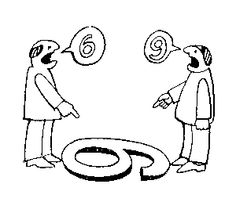
\includegraphics[width=0.49\linewidth]{./img/perceptuel.jpg} 
  \caption {Illustration du fait que deux individus peuvent avoir une interprétation divergente de l'environnement en fonction de leur situation spatiale. La capacité de comprendre que l'autre a une vision différente est liée à la prise de perspective perceptuelle (ou prise de perspective de niveau un).}
  \label{fig:perceptuel}
\end{figure}

La prise de perspective conceptuelle va plus loin et désigne la capacité d'un humain à attribuer des croyances et des sentiments aux autres\cite{Baron1985}.
Ainsi, dans l'illustration faite dans la figure \ref{fig:conceptual}, Bob fait une supposition sur l'état de croyance d'Alice concernant la contenance de la boîte.
Cette supposition que Bob fait de l'état de croyance d'Alice peut différer de l'état réel.

\begin{figure}[ht!]
 \centering
  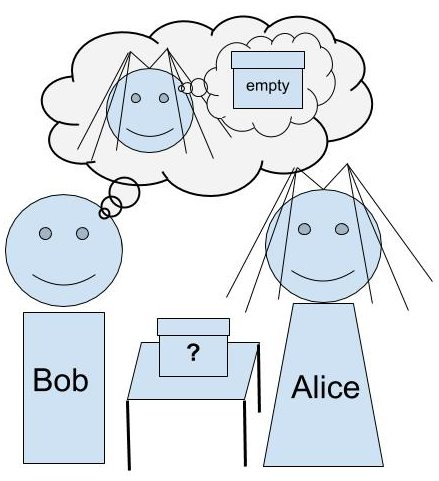
\includegraphics[width=0.49\linewidth]{./img/conceptual.jpg} 
  \caption {Illustration de la prise de perspective conceptuelle. Ici Bob attribue une croyance à Alice concernant la contenance de la boîte. Il suppose qu'elle croit que la boîte est vide. Cette faculté d'imputer des croyances aux autres s'appelle la prise de perspective conceptuelle (ou prise de perspective de niveau deux).}
  \label{fig:conceptual}
\end{figure}

Ainsi, dans la psychologie développementale, la faculté de comprendre qu'un autre puisse avoir une croyance erronée sur l'environnement qui l'entoure est considérée comme une étape importante dans l'évolution et l'acquisition de la théorie de l'esprit. Dans la littérature psychologique, la tâche de reconnaissance de fausse croyance ("false belief task" en anglais) a été formulée dans \cite{Wimmer1983103}. Heinz Wimmer et Josef Perner définissent un test (le test de Sally et Anne) qui permets d'évaluer les aptitudes d'une personne à comprendre qu'autrui possède des états mentaux différents des siens. Le test a été par la suite réalisé par Simon Baron-Cohen et Alan M. Leslie et rapporté dans \cite{Baron1985} et une seconde version dans \cite{Leslie1988}. Ce test est expliqué dans la figure \ref{fig:sallyAndAnne}.

%TODO Put it in Annexe?
\begin{figure}[ht!]
 \centering
  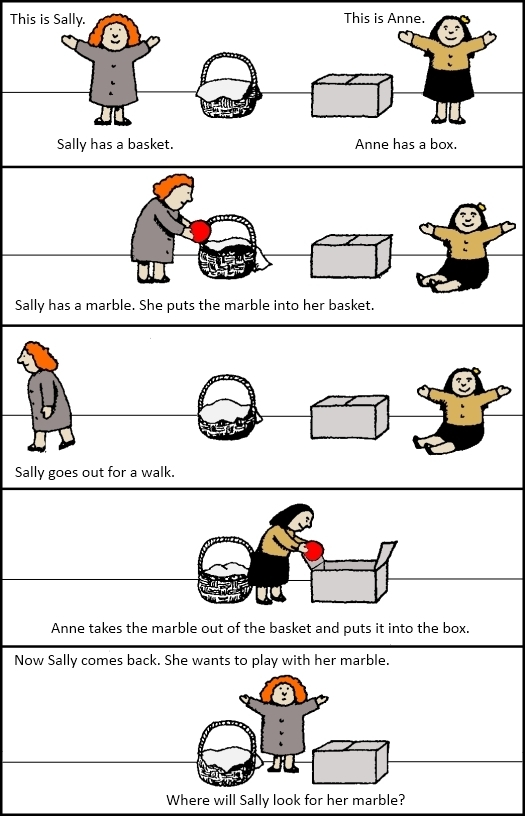
\includegraphics[width=0.89\linewidth]{./img/sally.jpg} 
  \caption {Test de Sally et Anne permettant de vérifier la capacité d'un individu à identifier un état de connaissance erroné chez autrui.}
  \label{fig:sallyAndAnne}
\end{figure}


%Perspective Taking is a human ability which allows one to see things from other's point of view. 
% Studied in
% psychology literature~\cite{Flavell1992,Tversky1999}, this ability is
% crucial when interacting with people by allowing one to reason on
% others' understanding of the world in terms of visual perception, spatial
% descriptions, affordances and beliefs, etc.
% Therefore, in the last years it has been gradually
% employed in Human-Robot Interaction. ~\cite{breazeal2006} presents a learning algorithm that takes into account information about a
% teacher's visual perspective in order to learn a task. ~\cite{Johnson2005} apply visual perspective taking for action
% recognition between two robots.~\cite{Trafton2005} use both visual
% and spatial perspective taking for finding out the referent
% indicated by a human partner.

% In psychology, Theory of mind (ToM) is defined as an understanding of other people’s mental states (their thoughts, feelings, desires, motivations, intentions).
% It includes perspective taking ability. Visual perspective
% taking is one of the most significant ToM precursor. 
% ToM encompasses a wide range of skills from instantaneous visual
% perspective skill to complex interpretation of other agent intents, plans,
% feelings occurring on a long time period.
% Increased ToM skills directly lead to increased performance when interacting
% with other agent in a collaborative as well as a competitive context.
% Being able to attribute false belief (to recognize that someone else
% has different beliefs about the physical world) has been considered
% as a milestone in ToM development.
% In psychology literature the false belief task was formulated in
% \cite{Wimmer1983103}.
% Breazal in ~\cite{BreazealGB09} proposed one of the first human robot
% implementation and proposed some more advanced goal recognition skills
% relying on this false belief detection.


% This paper will present an evolution of the previous work \cite{Warnier2012a} \cite{Lemaignan2012} \cite{Sisbot2011} with a refined management of divergent beliefs, temporal reasonning on data and improved inferring capabilities.
% These improvements allow the robot to pass Sally and Anne test \cite{Baron1985} (see Section IV B), to make inferences not only on position properties but also on dialogue, and other human actions.

% %%%%%%%%%%%%%%%%%%%%%%%%%%%%%%%%%%%%%

% ROMAN TOASTER 2016

\subsection{Usage en robotique}

Comme indiqué dans la partie \ref{sec:motivation}, pouvoir percevoir et raisonner sur l'environnement qui l'entoure sont des capacités nécessaires pour le robot mais non suffisantes lorsqu'il interagit avec des humains. Pour pouvoir comprendre la situation de l'humain, des recherches récentes ont tenté d'implémenter une sorte de théorie de l'esprit, en permettant au robot d'avoir la faculté de prise de perspective de niveau un (perceptuelle). Cynthia Breazeal présente dans \cite{breazeal2006} un algorithme d'apprentissage qui prends en compte l'information concernant le point de vue visuel de l'instructeur afin d'apprendre convenablement une tâche. Dans \cite{Johnson2005}, les auteurs appliquent la prise de perspective visuelle pour la reconnaissance d'action entre deux systèmes robotiques. Gregory Trafton dans \cite{Trafton2005} utilise à la fois la prise de perspective visuelle et spatiale pour identifier le référent indiqué par un partenaire humain. Dans \cite{ros2010one} la prise de perspective visuelle est utilisée pour simplifier la clarification de déclarations référentielles (referential utterances) dans des scénarios impliquant plusieurs objets.

Pour pleinement comprendre et se faire comprendre par l'homme, certaines études ont également visé à donner le niveau deux (conceptuel) de prise de perspective au robot. Cynthia Breazal dans ~\cite{BreazealGB09} propose l'une des première implémentation faisant intervenir un humain et un robot ainsi que quelques capacités plus avancées de reconnaissance de but basé sur cette détection de fausse croyance.
%TODO Compléter la biblio sur le niveau 2
%use: http://www.csc.kth.se/~hedvig/publications/cogsci_16.pdf

%%%%%%%%%%%%%%%%%%%%%%%%%%%%%%%%%%%%%%%%%%%%%%%%%%%%%%%%%%%%%%%%%%%%%%%
% This paper will present an evolution of the previous work \cite{Warnier2012a} \cite{Lemaignan2012} \cite{Sisbot2011} with a refined management of divergent beliefs, temporal reasonning on data and improved inferring capabilities.
% These improvements allow the robot to pass Sally and Anne test \cite{Baron1985} (see Section IV B), to make inferences not only on position properties but also on dialogue, and other human actions.

%ROMAN2014
% Secondly, it must be able to gain explicit reasoning on the human it
% interacts with. It means that not only the knowledge must be
% grounded between the robot and its interactor but also that the robot
% must be able to maintain an explicit representation of the knowledge
% of its interactor apart of its own knowledge. That will allow the
% robot to compare its own beliefs with the one of the human and to
% infer similarities as well as differences and ambiguities. Thus, the
% robot must be able to handle a kind of "theory of mind" \footnote{\url{http://en.wikipedia.org/wiki/Theory\_of\_mind}}.


% Equipped with such capabilities, a robot who will interact
% with humans should be able to extract, compute or infer these
% relations and capabilities in order to communicate and interact efficiently in a natural way.

% To achieve this we identified 3 main ingredients.
% First, the consideration of perspective-taking, i.e. the ability of
% the robot not only to build a model of the world for itself but
% also to estimate what its human partners perceive.
% Secondly, the ability to compute efficiently affordances for itself
% and to estimate the affordances of its human partners in a given situation 
% Finally, the ability to
% maintain a history of beliefs based on presence and focus of attention of humans which will enable reasoning on divergent beliefs.
% We will present how these features are implemented in SPARK as a permanent activity based on inter-related processes.


%%%%%%%%%%%%%%%%%%%%%%%%
% TOASTER ROMAN2016

% To make robots more socially competent, some research aims to endow robots with this ability.
% Some robotic research use the first level to have a better understanding of the human and remove ambiguities ~\cite{Trafton2005}, ~\cite{breazeal2006}, ~\cite{ros2010one}
% %B conceptual
% Concerning level two, various research on human robot interaction already aim to represent the human belief state.
% Breazal et al.~\cite{BreazealGB09} proposed one of the first human-robot implementation. In our previous work \cite{Milliez2014}, we made a primitive implementation to solve the Sally and Anne test described by Wimmer in~\cite{Wimmer1983}. In this primitive implementation, the reasoning on others belief state was limited to object position. We propose here a more generic approach to represent any kind of belief the human may hold on the environment.



%%%%%%%%%%%%%%%%%%%%%%%%%%%%%%%%%%%%%%%%%%%%%%%%%%%%%%%%%%%%%%%%%%%%%%

\section{Prise de perspective et état mental}

\subsection{Prise de perspective perceptuelle}
\label{sec:perceptuelle}

Dans notre système, pour donner au robot la capacité de se mettre à la place de l'homme et de comprendre ce qu'il est capable de percevoir et les éléments qui sont à sa porté, nous avons ajouté le calcul de deux faits basés sur la représentation tridimensionnelle de l'état du monde expliquée au chapitre précédent. Le premier permet de connaître ce qui est visible par l'homme, c'est à dire ce qui se trouve dans son champs visuel et n'est pas caché (ou tout du moins qui est suffisemment visible).

% To estimate what is visible for a human, it computes which objects are present in a cone, emerging from human's head. 
% If the object can be directly linked to the human's head with no obstacle and if it is in the field of the view cone, 
% then we assume that the human sees the object and hence has knowledge of its position. 
% If an obstacle is occluding the object, then it won't be visible for the human. 
% Concerning the reachability, a threshold of 1 meter is used to determine if the human can reach an object or not.


Ainsi, dans la figure \ref{fig:occludedHuman}, l'humain en bleu est incapable de voir l'objet à droite (\textit{WHITE\_BOOK}) car il est caché par la boîte grise (GREY\_BOX). Le système robotique est capable, en utilisant la position de la tête de l'homme et le modèle de l'environnement, de savoir quels objets sont visibles de l'homme et quel pourcentage de l'objet est visible.
En utilisant ce pourcentage, le système peut générer un fait concernant la visibilité de l'objet avec une confidence associée. Par exemple ici, le fait serait:

\begin{scriptsize}
\begin{verbatim}

Subject   property  target    value

ROBOT     canSee  WHITE_BOOK  true
HUMAN     canSee  WHITE_BOOK  false
\end{verbatim}
%\end{small}
%\end{footnotesize}
\end{scriptsize}

%TODO: surligné l'objet occlut
\begin{figure}[ht!]
 \centering
  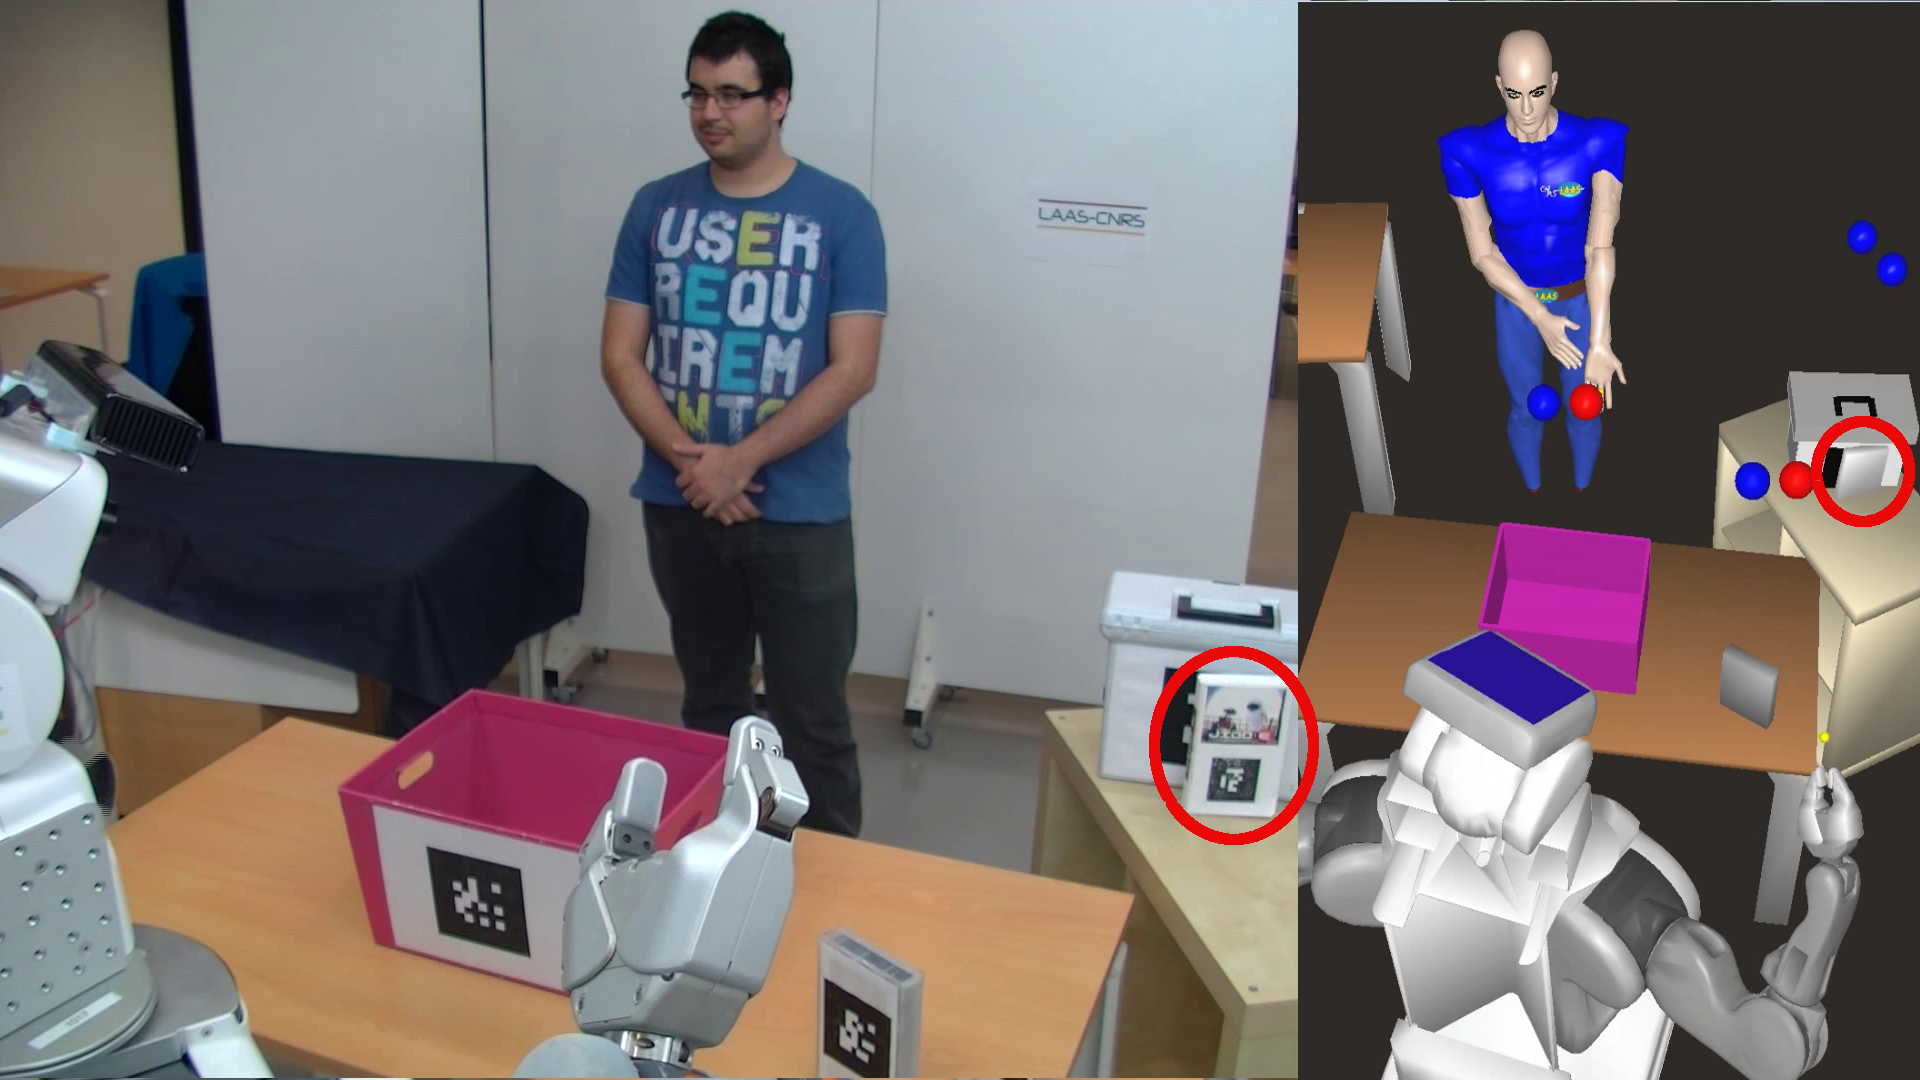
\includegraphics[width=0.99\linewidth]{./img/blueMovedPr2M.png} 
  \caption {Exemple d'état du monde où le système est capable de calculer la visibilité des objets pour chaque agent. Ici, le livre blanc n'est pas visible par l'homme.}
  \label{fig:occludedHuman}
\end{figure}


Le robot est donc capable de savoir ce qu'il est capable de percevoir (moyennant éventuellement un mouvement de tête), mais également ce que l'homme peut ou non percevoir. Nous verrons dans le chapitre suivant comment cela peut être utilisé durant une interaction, notamment pour améliorer le dialogue situé en terme d'efficacité.

Le second fait ajouté concerne le calcul permettant de savoir si les objets qui entourent l'homme sont à sa porté. En utilisant la bibliothèque 3D Move3D  \cite{Simeon2001}, il est en effet possible de calculer la cinématique d'un agent et de planifier ses mouvements. Grâce à cela, il est donc possible de savoir quels objets sont accessibles aux agents de la scène. Ce calcul est illustré par l'image \ref{fig:reach}, où le robot calcul l'accessibilité d'un objet par rapport à lui même et à l'homme présent dans la scène.



\begin{figure}[ht!]
 \centering
  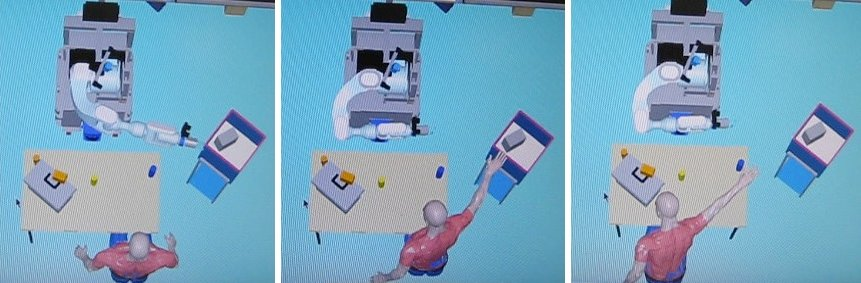
\includegraphics[width=0.99\linewidth]{./img/reach.jpg} 
  \caption {Exemple d'état du monde où le système calcul si les agents sont capables d'atteindre un objet. Sur l'image de gauche, le robot est capable de calculer qu'il peut attraper l'objet gris. Il calcul également que l'homme peut attraper l'objet gris, comme illustré par l'image centrale. Si l'homme avait été placé plus loin, le robot aurait pu calculé que l'objet était inaccessible pour l'homme, comme illustré par l'image de droite.}
  \label{fig:reach}
\end{figure}


La liste des faits (simplifiés) générés pour cette scène concernant l'accessibilité de l'objet gris serait pour les différentes configurations:

\begin{scriptsize}
\begin{verbatim}
left and center pictures                   right picture

Subject   property  target    value        Subject   property  target    value

ROBOT     canReach  GREY_OBJ  true         ROBOT     canReach  GREY_OBJ  true
HUMAN     canReach  GREY_OBJ  true         HUMAN     canReach  GREY_OBJ  false
\end{verbatim}
%\end{small}
%\end{footnotesize}
\end{scriptsize}

Pouvoir connaître quels objets sont à la porté de l'homme permets au robot de générer des plans collaboratifs prenant en compte cette donnée pour l'allocation de tâche, comme dans \cite{gharbi2015}.
Par exemple, si la tâche collaborative est de ranger des livres dans une boîte, si on a les faits:

\begin{scriptsize}
\begin{verbatim}

Subject   property  target     value

ROBOT     canReach  BLUE_BOOK   true
ROBOT     canReach  WHITE_BOOK  false
ROBOT     canReach  BASKET      false
HUMAN     canReach  BLUE_BOOK   false
HUMAN     canReach  WHITE_BOOK  true
HUMAN     canReach  BASKET      true
\end{verbatim}
%\end{small}
%\end{footnotesize}
\end{scriptsize}

le plan généré prendra en compte que le livre bleu (BLUE\_BOOK) et le panier (BASKET) sont atteignables par le robot pour lui assigner la tâche de ranger ce livre. De même, comme le livre blanc (WHITE\_BOOK) et le panier sont atteignables par l'homme, la tâche de le ranger lui sera assignée.
Ce fait peut également aider à la désambiguïsation, par exemple si l'homme demande au robot d'amener un objet, il est peu probable que l'homme parle d'un objet qui soit à sa porté.

%mais également comprendre la situation de l'homme avec lequel il intéragit.
Pour comprendre l'homme, il est également important de comprendre sa situation spatiale, à savoir comment celui-ci est entouré et comment il est susceptible de décrire ce qui l'entour par rapport à sa position.

Nous avons donc ajouté dans notre système d'évaluation de la situation la possibilité de faire des requêtes pour obtenir la position d'une entité du point de vue d'un agent. Il est par exemple possible de calculer de quel côté une entité se trouve (gauche, droite, avant, arrière).
De plus, il est aussi possible d'obtenir la position d'une entité comparativement à une autre du point de vue d'un agent. Par exemple, il est possible pour le robot de dire à l'homme "la tasse que vous cherchez est \textbf{à votre droite}" ou "Donnez moi le livre qui est \textbf{pour vous à gauche de la tasse rouge}".
Ces requêtes permettent donc au robot d'avoir une prise de perspective géométrique et ainsi de parler à l'homme en prenant son propre référentiel, améliorant ainsi les performances sociales du robot.

\begin{figure}[ht!]
 \centering
  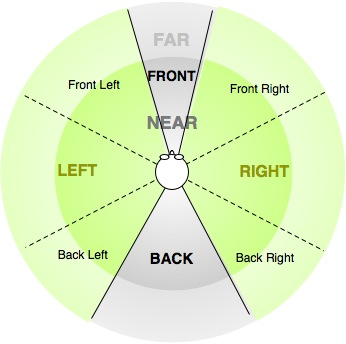
\includegraphics[width=0.59\linewidth]{./img/relative_position.jpg} 
  \caption {Illustration du découpage géométrique pour désigner les emplacements en prenant l'homme comme référentiel.}
  \label{fig:relativePose}
\end{figure}


\subsection{Prise de perspective conceptuelle}
\label{sec:beliefm}
\subsubsection{Modélisation des états mentaux}
Nous avons expliqué dans le chapitre \ref{chapter1} qu'il est important de faire des hypothèses sur la position des objets pour pouvoir en assurer le suivi. Bien que nécessaire, le fait de créer des hypothèse implique la possibilité de se tromper.
%En conclusion du chapitre 2, nous avons expliqué comment il est possible de probabiliser l'état du monde pour prendre en compte l'incertitude du robot.
Dans cette section nous allons expliquer comment la prise de perspective va permettre au robot d'avoir connaissance de l'état de croyances des hommes avec lesquels il interagit et ainsi savoir lorsqu'ils ont une croyance erronée concernant l'environnement.

La première étape pour pouvoir connaître l'état mental d'un humain est d'avoir connaissance des informations qu'il reçoit. L'humain peut recevoir des informations sur son environnement de deux façons: soit il les reçoit directement (ou les déduit) de ses capacités perceptives, soit il les reçoit d'un autre agent à travers le dialogue.
Pour donner au robot la capacité de prise de perspective décrite en \ref{sec:psy}, nous nous focalisons dans un premier temps sur la perception et sur le dialogue homme-robot pour déduire quelles informations l'humain peut acquérir.

Grâce aux calculs des affordances des agents expliqués en \ref{sec:perceptuelle}, il est possible de savoir lorsqu'un agent perçoit un objet. Lorsqu'un humain voit un objet, cela implique qu'il acquiert la connaissance de sa localisation, et donc mets à jour cette information dans son état d'esprit. Cela permets donc de suivre l'état de connaissance de chaque agent.

L'état mental de chaque agent (tel qu'il est estimé par le robot) est ainsi conservé et mis à jour dans un modèle séparé de l'état de connaissance que le robot lui-même possède sur l'environnement. Ainsi, le modèle représentant l'état mental de chaque agent se traduit par une liste de faits. Chaque modèle est indépendant et cohérent d'un point de vu logique.

%TODO speak about database implementation?

% In SPARK we have the position of humans (see III 1.). We use it to
% calculate affordances of each human toward elements of the scene he can interact with.
% To estimate what is visible for a human, it computes which objects are present in a cone, emerging from human's head. 
% If the object can be directly linked to the human's head with no obstacle and if it is in the field of the view cone, 
% then we assume that the human sees the object and hence has knowledge of its position. 
% If an obstacle is occluding the object, then it won't be visible for the human. 
% Concerning the reachability, a threshold of 1 meter is used to determine if the human can reach an object or not.

%comment peut etre mettre un exemple de modèle d'agent,
%  même tout petit pour mettre les idées en place ?}


\subsubsection{Gestion de croyance divergente}
\label{sec:divB}
Dans certains cas, l'homme et le robot peuvent avoir un modèle qui contient des valeurs différentes. Cela peut provenir d'une vision différente de la scène (e.g. certaines propriétés sont accessibles uniquement au robot, donc l'homme n'en a pas connaissance).
Cela peut provenir de croyances divergentes entre l'homme et le robot (e.g. l'homme croit qu'un objet a la propriété \textit{P} alors que le robot sait que cette propriété est fausse). Dans ce second cas, la prise de perspective n'est pas suffisante pour comprendre la croyance erronée de l'homme. Il est nécessaire de mettre en place la gestion de croyance divergente (divergent belief management en Anglais).


% This Management relies on data from the environment as well as from
% affordances and supervisor.
% This way, the robot can generate beliefs according to the task stated in correlation with  affordances 
% as shown in fig. ~\ref{beliefs_fg}.

% \begin{figure}[ht!]
%  \centering
%   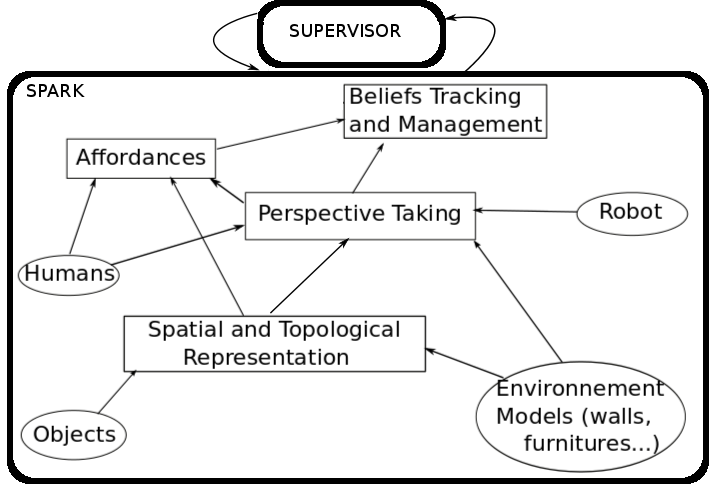
\includegraphics[width=0.99\linewidth]{./img/beliefs2.png} 
%   \caption {Schema of SPARK reasoning to generate beliefs}
%   \label{beliefs_fg}
% \end{figure}
Par exemple, si on considère qu'un humain appelé \textit{GREG} quitte la zone d'interaction avec la croyance qu'un objet \textit{Obj} a la propriété \textit{Prop} dans un état \textit{e1}. 

On présente ci-dessous l'état de connaissance du robot et celui de \textit{GREG} tel qu'il est modélisé par le robot.

\begin{scriptsize}
\begin{verbatim}
          ROBOT                  GREG
      Obj Prop e1            Obj Prop e1
\end{verbatim}
%\end{small}
%\end{footnotesize}
\end{scriptsize}

Durant son absence, imaginons que la propriété \textit{Prop} appliquée à \textit{Obj} a évolué pour atteindre un état \textit{e2}.
Lorsque \textit{GREG} revient, même si la propriété a évolué, il pensera probablement que la propriété est dans le même état que lorsqu'il a quitté la scène, jusqu'à ce qu'il soit capable de réévaluer ses croyances en utilisant le dialogue ou la perception. Pour prendre en compte ce type de situation, le robot garde inchangé le modèle d'un agent lorsque celui-ci n'est pas présent pour observer les actions ou constater les changements induits, et ce jusqu'à son retour.

Avant que l'homme ne revienne, la croyance du robot a donc évoluée mais pas celle de l'homme.

\begin{scriptsize}
\begin{verbatim}
          ROBOT                  GREG
      Obj Prop e2            Obj Prop e1
\end{verbatim}
%\end{small}
%\end{footnotesize}
\end{scriptsize}

Lorsque l'homme revient, on identifit trois situations différentes:

%%%%%%%%%%%%%%%%%%%%%%%%%%%%%%%%%%%%%%%%%%%%%%%%%%%%%%%%%%%%%%%%%%%
%illustrate each situation with images
\begin{itemize}
\item Dans le premier cas, l'homme remarque le changement d'état de la propriété et corrige directement sa croyance erronée. Le robot corrige donc automatiquement le vecteur de faits représentant les croyances de \textit{GREG} avec le nouvel état de la propriété. 

%illustrate each situation with images

\begin{scriptsize}
\begin{verbatim}
          ROBOT                  GREG
      Obj Prop e2            Obj Prop e2
\end{verbatim}
%\end{small}
%\end{footnotesize}
\end{scriptsize}


Pour illustrer, on peut prendre comme objet une radio (\textit{RADIO}) et comme propriété l'état (\textit{turnedOn}) qui peut avoir comme valeur allumée (\textit{TRUE}) ou éteinte (\textit{FALSE}). Si \textit{GREG} quitte la scène en sachant que la radio est allumée, lorsqu'il revient, n'entendant plus la radio, il pourra directement déduire la nouvelle valeur de la propriété d'état liée à la radio (éteinte).

%illustrate each situation with images

\begin{scriptsize}
\begin{verbatim}
          ROBOT                  GREG
    RADIO turnedOn FALSE   RADIO turnedOn FALSE
\end{verbatim}
%\end{small}
%\end{footnotesize}
\end{scriptsize}


\item La deuxième situation, l'homme remarque le changement mais est dans l'incapacité de connaître le nouvel état de la propriété. L'humain étant au courant de son ignorance, le robot supprime sa croyance erronée. Pour ce faire, il mets à jour le vecteur de faits avec un état \textit{unknown} qui traduit le fait que le robot ait connaissance que l'homme sait qu'il ignore le nouvel état de la propriété.


\begin{scriptsize}
\begin{verbatim}
          ROBOT                  GREG
      Obj Prop e2            Obj Prop unknown
\end{verbatim}
%\end{small}
%\end{footnotesize}
\end{scriptsize}



On peut prendre cette fois comme exemple un livre (\textit{BOOK}) ayant comme propriété une position (\textit{isOn}) et pouvant avoir pour valeur le meuble sur lequel il se trouve (\textit{LIVINGROOM\_TABLE}, \textit{BEDSIDE\_TABLE}, \textit{BEDROOM\_SHELF}). Si \textit{GREG} quitte la scène en sachant que le livre est sur la table du salon, lorsqu'il revient, s'il observe que le livre n'est plus à sa place, il aura alors connaissance que la propriété de position a changé de valeur sans être capable de savoir la nouvelle valeur de celle-ci tant qu'il n'aura pas vu l'objet.

\begin{scriptsize}
\begin{verbatim}
          ROBOT                         GREG
     BOOK isOn LIVINGROOM_TABLE    BOOK isOn unknown
\end{verbatim}
%\end{small}
%\end{footnotesize}
\end{scriptsize}



\item Dans la troisième situation, l'homme est incapable de remarquer que la propriété a changé. L'humain va alors garder sa croyance erronée concernant la propriété jusqu'à ce qu'il puisse constater un changement ou que le robot l'informe de l'évolution de la propriété. 

\begin{scriptsize}
\begin{verbatim}
          ROBOT                  GREG
      Obj Prop e2            Obj Prop e1
\end{verbatim}
%\end{small}
%\end{footnotesize}
\end{scriptsize}

Pour prendre un dernier exemple, si l'objet est une boîte de cookies (\textit{COOKIE\_BOX}) opaque et que la propriété décrit la présence de cookies à l'intérieur de la boîte (\textit{isFull}), pouvant prendre pour valeurs pleine (\textit{TRUE}) ou vide (\textit{FALSE}). Si lorsque \textit{GREG} quitte la scène il pense que la boîte est vide, si celle-ci a été remplit pendant son absence, \textit{GREG} sera incapable de savoir que la boîte est à présent remplie tant que celle-ci sera fermée (et donc l'état de la propriété \textit{isFull} non observable).

\begin{scriptsize}
\begin{verbatim}
           ROBOT                         GREG
COOKIE_BOX isFULL TRUE        COOKIE_BOX isFULL FALSE
\end{verbatim}
%\end{small}
%\end{footnotesize}
\end{scriptsize}
\end{itemize}

%%%%%%%%%%%%%%%%%%%%%%%%%%%%%%%%%%%%%%%%%%%%%%%%5





% Knowing these beliefs is a great help to the robot to understand human and interact with him.
% The robot takes human's perception into account to have appropriate interpretation of human requests, to proactively inform or warn the human about a missing or wrong belief and also to generate a collaborative plan. 
% Thus, the robot has to reason on what a human can see, reach and
% knows to get these skills.




%%%%%%%%%%%%%%%%%%%%%%%%%%%%%%%%%%%%%%
% ROMAN2016 INTENTION
% We consider our world as a dynamic environment, where entities can move, objects' properties can change and actions can be performed.  We define an action as a tuple $(name, preconditions, target, postconditions)$. The $name$ of an action is a unique string that identifies it. The $preconditions$ are a list of properties that must be true in order to realize the action. In our system, an action is executed on a $target$, which can be a physical object, like a cup, but also an area of the environment, like a room. The $postconditions$ are the set of properties, and their values, affected by the action's execution.

% Since we are interested, in this paper, on reasoning and not perceptual aspects, we use inference, as explained in Sec. \ref{sec:intention_recognition}, in order to understand when a human has performed an action. Through the predefined $postconditions$ of actions we can also infer changes in object properties, e.g. the human opens a box, so the box is now open. 

% Since the environment is dynamic, agents can have divergent representations of the world. To model this aspect, the information produced by perception, geometrical reasoning and inference, are collected by the robot in \textit{belief models}, built for itself and for each agent. A \textit{belief model} is a symbolic representation of the world state, as known by an agent. In a model, the world state is represented by properties and values. To represent the lack of knowledge of an agent, the value of a property can be \textit{unknown}.
% We created a rule based framework in order to build beliefs of each agent and update them when needed. Human belief models are updated using the perspective taking skills of the robot. When the robot detects the execution of an action in the world, it updates the belief model for itself and for every human that can perceive the action, adding the action's $postconditions$ to their models. When an action is not perceived by a human (e.g. the user was in an other room), his belief model won't be updated, as he is not aware of the changes that occurred.



\section{Implémentation}
\label{sec:dbPt}
%BASE DE DONNÉE
%(Implémentation)

\subsection{Traitement générique de la mise à jour de l'état de croyance}
Pour pouvoir avoir un état du monde symbolique pour chaque agent afin de représenter la conception mentale que celui-ci a de l'environnement, il est possible d'ajouter une table dans la base de données temporelle.
Cette table est comparable à la table \textit{ROBOT\_WS\_TBL} décrite en section \ref{sec:dbd} et qui contient une liste de faits décrivant l'état du monde perçu par le robot lui-même.
De même que cette table contenant la représentation symbolique de l'environnement par rapport à l'état mental d'un agent tel qu'il est estimé par le robot, nous ajoutons également une table mémoire pour chaque agent. Cette table représente l'état de croyance passée de l'agent courant. Elle est comparable à la table \textit{ROBOT\_MEM\_TBL} décrite en section \ref{sec:dbt}.

Cependant, pour le robot la mise à jour de ces tables repose directement sur la perception de l'environnement basée sur les différents modules de TOASTER décrits en section \ref{sec:calculs} et sur le module de gestion des hypothèses décrit en section \ref{sec:hypo}. Pour pouvoir mettre à jour les croyances de l'homme, il faut pouvoir mettre en place une gestion des croyances tel que décrite en section \ref{sec:divB}.

Pour se faire, comme expliqué en section \ref{sec:divB}, lorsqu'un agent ne peut percevoir un événement, son état mental reste inchangé.
Toute la difficulté ici est de parvenir à estimer lorsque l'homme est capable ou non de mettre à jour son état de croyance.
En effet, selon la propriété concernée, l'état peut être plus ou moins observable ou inférée selon divers moyens de perception.

Par exemple, la propriété de localisation d'un objet est une propriété directement observable. En effet, si un homme observe un objet, il aura directement la connaissance de sa position. Par contre, si l'on reprend l'exemple de la boîte de cookies, l'observabilité de la propriété de contenance dépends de la propriété relative à l'ouverture de cette boîte. Ainsi, il est possible d'observer la contenance de la boîte de cookie seulement si celle-ci est ouverte.
De plus, la perception peut passer par divers modalité. Par exemple pour savoir qu'une tasse est chaude il est possible soit de percevoir de la fumée émanant de la tasse, soit de ressentir la chaleur de celle-ci dans la main.
Enfin, l'observabilité est également liée aux capacités de perception de chaque agent. Ainsi, si l'on reprend l'exemple de la radio, une personne sourde ne sera pas en capacité de savoir si celle-ci est allumée ou éteinte.

Afin de proposer une première implémentation et de mettre en place une gestion générique des hypothèses et du maintien de l'état mental de chaque agent, nous avons ajouté à chaque fait une notion d'observabilité, correspondant au champ \textit{factObservability} déjà présenté en section \ref{sec:facts} lors de la présentation de la structure de \textit{fait}.
L'observabilité représente la probabilité qu'un agent puisse acquérir l'état d'une propriété lorsque le sujet (\textit{subject}) du fait est visible.

Pour gérer la mise à jour nous utilisons les règles suivantes qui sont une adaptation des règles énoncées en section \ref{sec:divB}. 
Nous appelons $H$ l'agent, $HB$ son modèle de croyance, et $RB$ le modèle de croyance du robot. Nous créons également les prédicats suivants: $obs(p)$ signifie que l'instance de la propriété $p$ est observable, et probObs(p) l'observabilité de la propriété comme définie précédemment. $valid(p,x)$ signifie que l'instance de la propriété $p$ ne contredit pas la perception courante de l'agent $x$. $value(p,m)$ est la valeur du prédicat $p$ dans le modèle de croyance $m$, et $vis(p,x)$ signifie que l'agent $x$ est capable de voir (lié à la propriété \textit{canSee} évoqué en section \ref{sec:perceptuelle}) l'entité sujet de la propriété $p$. $conf(p,x)$ représente la confiance que le robot a dans le fait que $x$ ait effectivement mis à jour la valeur de la propriété $p$. L'évaluation de la validité d'un prédicat étant hautement variable, il n'a été implémenté pour l'instant que pour les propriétés de position. En effet, pour les propriétés de position, le fait de pouvoir observer l'emplacement précédent suffit à savoir que la propriété n'est plus valide.
Nous avons donc l'ensemble des règles de mise à jour suivant, pour chaque propriété  $p\in HB \cup RB$: 



% We call $H$ the agent, $HB$ his belief model, and $RB$ the robot's belief model. We also create the following predicates: $obs(p)$ means that the instance of property $p$ is observable, $valid(p,x)$ means that the instance of property $p$ doesn't contradict the current perception data of agent $x$, $value(p,m)$ is the value of predicate $p$ in belief model $m$, and $vis(p,x)$ means that agent $x$ has visibility on the linked entities of property $p$. The rules for the $valid$ predicate will be different in each property. For example the property \textit{MUG isOn TABLE} won't be valid for agent Max if he can see that there is no mug on the table. For each property $p\in HB \cup RB$:
\begin{itemize}
\item if $p \in RB, \quad p\not\in HB,\quad obs(p),\quad vis(p,H) \rightarrow value(p,HB)=value(p,RB)$.
\item if $p \not \in RB,\quad p\in HB,\quad obs(p),\quad vis(p,H) \rightarrow remove\quad $p$ \quad from \quad HB$.
\item if $p\in RB,\quad p\in HB$ then:
	\begin{itemize}
      \item if $value(p,HB)\neq value(p,RB),\\ \quad obs(p),\quad vis(p,H) \rightarrow  value(p,HB)=value(p,RB)$ \\
      $conf(p,H)=vis(p,H)*probObs(p)$.
      \item if $value(p,HB)\neq value(p,RB),\\ \quad !obs(p),\quad !valid(p,H) \rightarrow  value(p,HB)=\textit{unknown}$.
	\end{itemize}
\end{itemize}

L'idée de cet ensemble de règle est de mettre à jour le modèle d'état mental d'un agent seulement si le sujet de la propriété est observable par l'agent concerné, ou si il n'est pas observable mais que les données de perception contredisent la valeur actuelle de la propriété (par exemple si un mug a été déplacé de la table de la cuisine à une étagère en l'absence de l'agent, même si l'agent ne peut voir où est le mug, il peut voir qu'il n'est plus sur la table).


\subsection{Réflexion sur d'éventuelles améliorations}
La méthode d'implémentation basée sur les règles définies ci-dessous permets un traitement "automatique" et générique des divers propriétés.
Cependant, cette implémentation est très simplifiée car comme indiqué précédemment, 
l'observation de l'invalidité d'une propriété ou l'acquisition du nouvel état d'une propriété peut être très variable d'une propriété à l'autre.

L'une des façons d'améliorer simplement les règles déjà existante serait de considérer l'observabilité d'une propriété non seulement en la basant sur la visibilité du sujet mais aussi de la cible pour certaines propriétés. Ainsi selon la propriété, la mise à jour de l'état pourrait être liée à la possibilité de voir le sujet ou la possibilité de voir la cible ou la possibilité de voir les deux à la fois.

Une autre façon d'améliorer la gestion des croyance serait de créer un ensemble de règle définissant les différents moyens de mise à jour d'une propriété.
Ainsi, pour le problème de la propriété de contenance de la boîte opaque, il faudrait vérifier que: la boîte est visible par l'agent, que son contenu est visible et que la boîte est ouverte.
Un autre exemple, pour savoir qu'un agent \textit{H1} est capable de savoir qu'un agent \textit{R} peut voir un objet \textit{O} il lui faut non seulement pouvoir voir la position de \textit{R} mais aussi connaître (ou voir) la position de l'objet \textit{O}.
Cette méthode, bien qu'envisageable nécessiterait de définir des règles pour chaque propriétés, ou tu du moins chaque type de propriétés, et donc nécessite de définir un domaine réduit avec des règles données au robot par un expert.
Un moyen d'éviter cela serait de développer des mécanismes d'apprentissage afin que le robot apprenne de lui-même ces règles.


%TODO finir: expliquer comment ça marche, ajouter des formules?
%observabilité subject / target?

%we assumed in previous chapter that perception object update property.
%However, for some properties visual, some different...
% We assume here that if the human is able to perceive an object property, he is then aware of the object property state. As an example for position property, if there is no obstacle between his eyes and the object and the object is in the human field of view, 
% he is then aware of its position.

%explain how we do -> observability
%explain that it is a first approximation, hypothesis are based on lot of things.
%confidence should shrink with time
%Database, cf roman 2016

%TODO: then detail how to update mental states: different for position hypothesis (sub symbolic) and other properties. observability Or maybe put it in implementation?
%Visual pereception -> position, light on...
%Some are not easily perceived by vision: hot, isFull...

\section{Résultats expérimentaux}
%Sally and Anne + experience améliorée, cf Roman 2014

%%%%%%%%%%%%%%%%%%%%%%%%%%%%%%%%%%%%%%%%%%%%%%%%%%%%%%%%%%%%%%%
Nous présentons ici l'une des expériences menée au LAAS permettant de mettre en valeur la capacité du système à maintenir et mettre à jour l'état mental des humains présents grâce aux mécanismes de suivi et de mise à jour d'état mental présenté précédemment.

\subsection{Configuration expérimentale}
\label{sec:chap2expconf}
Tout d'abord, nous présentons brièvement les capteurs et modules que nous utilisons pour les expérimentations.


Ces expérimentations ayant été réalisées en 2014, l'infrastructure logicielle utilisée pour l'estimation de la situation est SPARK\cite{Milliez2014}, qui est une version antérieure à TOASTER mais qui a un fonctionnement similaire pour le suivi de l'état mental des humains concernant les propriétés de position des objets.

%TODO: redo
\begin{figure}[ht!]
  \centering
  %% \includegraphics[width=0.7\textwidth]{./figs/supervisor-architecture-new.pdf} \\
% \includegraphics[width=0.5\textwidth]{./image/sparkinput.png} \\
 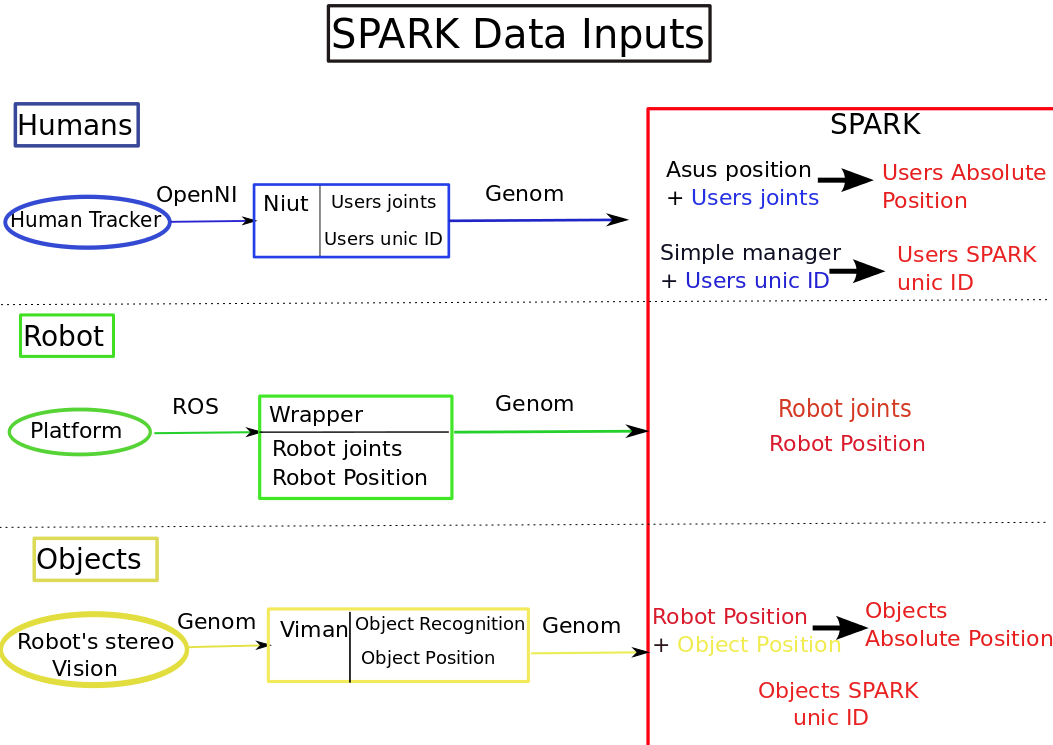
\includegraphics[width=0.99\linewidth]{./img/spark_input.png} 
  \caption {Schéma représentant les entrées de SPARK.}
  \label{fig:inputSpark}
\end{figure}

Pour assurer le suivi des humains, nous utilisons une Asus xtion. Comme le fait de bouger la tête est une partie importante de la communication pour permettre au robot de montrer son attention, et pour éviter la perte du suivi, nous avons fixé l'Asus xtion sur une base stable derrière le robot.
Un module, appelé \textit{niut}, est responsable de la gestion du suivi des humains, en utilisant l'API OpenNI. Ce module détecte également la teinte moyenne du haut des humains afin de les identifier. Pour obtenir la valeur moyenne de la teinte de chaque humain, on extrait la position du torse, puis nous la projetons dans les coordonnées de l'image RGB. Si les données sont disponibles, le module utilise également les coordonnées des épaules et des hanches pour définir le rectangle dans lequel la teinte sera calculée, sinon le module créé un rectangle au tour de la position du torse, en adaptant l'échelle en fonction de l'éloignement de l'humain.
En donnant au module les valeurs des teintes de chaque humains, il est possible de reconnaître l'humain et d'envoyer ses données de postures au module d'estimation de la situation avec un id unique. Cela permets également de filtrer les faux positifs dans la détection d'humains et évite que des humains non enregistrés perturbent le déroulement des expériences.
Pour que les hommes soient à la bonne position dans le modèle du monde, une projection est effectuée à partir de la position et l'orientation de l'Asus xtion.

La posture et la position du robot sont directement obtenues grâce à ses capteurs internes en utilisant l'intergiciel ROS.

Enfin, pour obtenir la position des objets, nous utilisons le module \textit{Viman} qui est basé sur la bibliothèque de réalité augmentée ARToolKit\footnote{http://artoolkit.org/}. Ce module utilise la vision stéréo du robot pour reconnaître et localiser les objets. Pour ce faire, \textit{viman} scan des RTags placés sur les objets.
Une fois que la position relative (à la caméra) de l'objet est connue, elle est envoyée au module d'estimation de la situation qui, en utilisant la position de la tête du robot pourra obtenir la position de l'objet dans le monde par projection.
La figure \ref{fig:inputSpark} illustre cette implémentation.


\subsection{Résultats}
\label{sec:ResChap2}


Nous avons introduit ci-dessus comment nous procédons pour suivre les croyances distinctes pour chaque agent. Nous croyons que cette fonctionnalité est utile pour comprendre la verbalisation de l'homme, ses actions et la focalisation de son attention, i.e. pour interagir avec des humains. Comme le robot connaît les croyances des humains il peut décider de quelle information est-il nécessaire de fournir à l'homme et également si il doit parler ou non en fonction de la situation actuelle ou de l'état de réalisation du plan collaboratif. La fonctionnalité de gestion de croyance présenté dans ce chapitre a été utilisée sur un robot afin de les tester \footnote{Des vidéos des expérimentations sont accessibles à l'url: \url{http://homepages.laas.fr/gmilliez/roman2014/}}.




\subsubsection{Le Test de Sally et Anne}

Pour aider à la compréhension des scénarios, la figure \ref{SA} et la figure  \ref{divB} sont des images de l'expérimentation réelle avec des captures d'écran de la modélisation 3D du module de raisonnement spatial.


\begin{figure*}[ht!]
  \begin{center}
    \subfigure[Greg (en vert) et Bob (en bleu) font face au robot. Ils connaissent la position de chaque objet.]{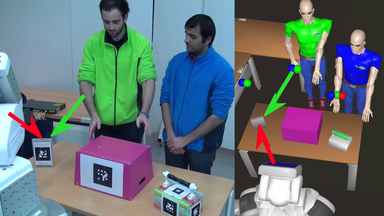
\includegraphics[width=0.49\textwidth]{./SallyAndAnne/1mas.png}\label{initSA}}
    \subfigure[Greg mets la boîte rose sur le livre blanc.]{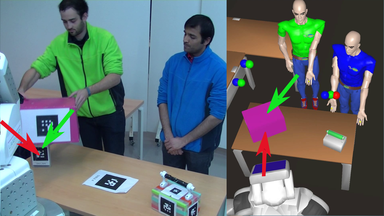
\includegraphics[width=0.49\textwidth]{./SallyAndAnne/2mas.png}\label{startSA}}
    \subfigure[Greg pars et Bob enlève le livre blanc de la boîte rose.]{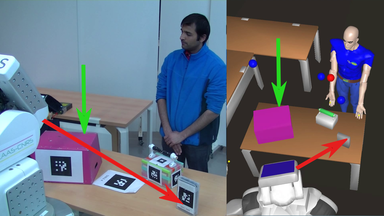
\includegraphics[width=0.49\textwidth]{./SallyAndAnne/3mas.png}\label{middleSA}}
    \subfigure[Bob mets le livre blanc sous la petite boîte, puis Greg revient. Le robot est capable de comprendre que Greg croit que le livre est sous la boîte rose.]{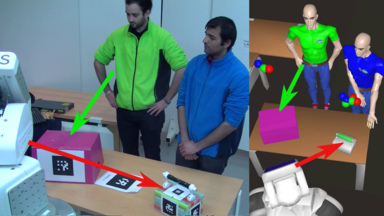
\includegraphics[width=0.49\textwidth]{./SallyAndAnne/4mas.png}\label{endSA}}
 \end{center}
  \caption{Le test de Sally et Anne dans l'environnement réel (partie de gauche) et tel qu'il est perçu par le robot (partie de droite). Pour aider à la compréhension, nous montrons explicitement les croyances concernant la position du livre blanc. Les croyances de Greg sont indiquées avec des flèches vertes et celles du robot avec des flèches rouges.
Les petites sphères de couleur dans l'environnement perçu sont utilisées comme des indications sur l'accessibilité d'un objet pour un agent.}
  \label{SA}
\end{figure*}

Dans le premier scénario, afin de tester notre système et d'illustrer l'habileté du robot à détecter les croyances fausses/divergentes sur la position d'un objet nous avons décider de le soumettre au test de Sally et Anne déjà présenté par la figure \ref{fig:sallyAndAnne}. Dans notre expérience, deux utilisateurs Greg (en vert) et Bob (en bleu) font face au robot
La scène est composée d'un livre blanc et de deux boîtes se trouvant sur une table \ref{initSA}).
Greg mets le livre blanc sous la boîte rose (\ref{startSA}). Puis Greg quitte la scène. Pendant que Greg est parti, Bob prends le livre blanc et le mets sous la petite boîte. (\ref{middleSA} et \ref{endSA}).
Puis, quand Greg revient, nous demandons au robot où Greg pense que le livre se trouve.





Nous allons présenter ci-dessous quelques faits symboliques intéressants pour Greg et le robot correspondant à la situation décrite en \ref{endSA}. Les croyances de Bob restent identiques à celles du robot et ne seront donc pas affiché par simplification.
\begin{scriptsize}
\begin{verbatim}
          ROBOT                         GREG
GREG canSee PINK_BOX  TRUE      GREG canSee PINK_BOX  TRUE
GREG canSee SMALL_BOX TRUE      GREG canSee SMALL_BOX TRUE
GREG canSee BOOK      FALSE     GREG canSee BOOK      FALSE
BOOK isIn   SMALL_BOX TRUE      BOOK isIn   PINK_BOX  TRUE

\end{verbatim}
\end{scriptsize}

Comme le robot sait que le livre n'est pas visible par Greg, il n'a pas mis à jour ses croyances concernant la position de cet objet. Avec l'aide du système d'estimation de la situation maintenant le modèle de croyance des agents, le robot est capable d'observer que, comme Greg ne peut observer ce qui a changé, il a une croyance divergente sur la position de l'objet. Si l'homme et le robot doivent accomplir une tâche impliquant cet objet, le robot sera capable de savoir qu'il doit informer l'homme de la position de l'objet.

\subsubsection{Gestion de croyance divergente}


Pour aller plus loin et illustrer les trois différentes situations présentées en section \ref{sec:divB}, nous avons tourné un autre scénario illustré par la figure \ref{divB}. Dans cette deuxième expérimentation, deux utilisateurs, Greg et Bob, font face au robot. Ils ont un livre blanc et une boîte blanche qui servira pour faire de l'occlusion visuelle (\ref{initDB}).
Une fois que Bob pars (\ref{startDB}) Greg prends le livre blanc et le mets derrière la boîte blanche pour qu'il ne soit pas visible du point de vue humain (\ref{startDB}).
Puis Greg pars et Bob revient. Le robot est capable de comprendre que, comme le livre blanc est caché, Bob ne sait pas où il se trouve. Toutefois, Bob peut voir que le livre n'est plus là où il pensait qu'il serait. Cette information manquante est représenté par une sphère transparente à l'emplacement où Bob pensait trouver l'objet (\ref{lackBobDB}).


\begin{figure*}[ht!]
  \begin{center}
    \subfigure[Greg (en vert) et Bob (en bleu) font face au robot. Ils connaissent la position de chaque objet.]{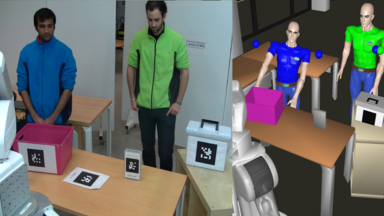
\includegraphics[width=0.49\textwidth]{./DivBFull/1ms.png}\label{initDB}}
    \subfigure[Bob pars, Greg mets le livre blanc derrière la boîte blanche.]{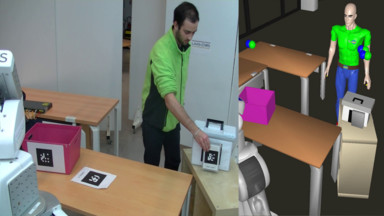
\includegraphics[width=0.49\textwidth]{./DivBFull/2ms.png}\label{startDB}}
    \subfigure[Greg pars et Bob revient. Bob ignore la position du livre blanc. Le robot est au courant de ce manque d'information (une sphère bleue transparente représente la dernière croyance de Bob concernant la position du livre blanc).]{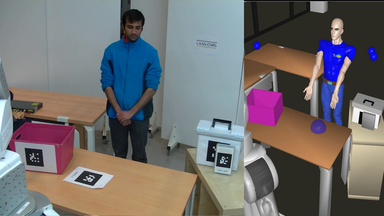
\includegraphics[width=0.49\textwidth]{./DivBFull/3ms.png}\label{lackBobDB}}
    \subfigure[Bob regarde derrière la boîte blanche (et donc mets à jour ses croyances) et prends le livre blanc. ]{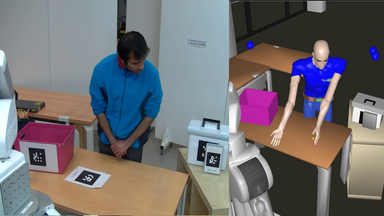
\includegraphics[width=0.49\textwidth]{./DivBFull/4ms.png}\label{updateBobDB}}
    \subfigure[Bob pars avec le livre blanc, puis Greg revient. Greg pense toujours que le livre blanc est derrière la boîte blanche. Le robot est au courant de cette croyance divergente (Une sphère opaque verte représente la croyance actuelle de Greg concernant la position du livre blanc).]{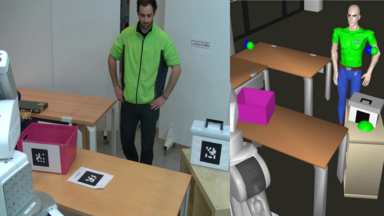
\includegraphics[width=0.49\textwidth]{./DivBFull/6ms.png}\label{GregDB}}
    \subfigure[Greg regarde derrière la boîte blanche et est alors informé que sa croyance est erronée mais ne connaît pas la nouvelle position de l'objet (la sphère devient transparente).]{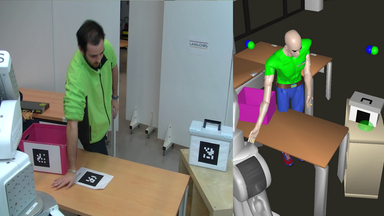
\includegraphics[width=0.49\textwidth]{./DivBFull/7ms.png}\label{lackGregDB}}
 \end{center}
  \caption{Scénario de croyance divergente impliquant un robot Pr2 et deux humains. Le robot est capable de modéliser les croyances de chacun. Les images présentes les étapes du scénario dans l'environnement réel (partie de gauche) et tel qu'il est perçu par le robot (partie de droite).}
  \label{divB}
\end{figure*}

Ci-dessous sont représentés quelques faits symboliques concernant les croyances de Bob et du robot tel que le robot les modélise.

\begin{scriptsize}
\begin{verbatim}
          ROBOT                                    BOB
ROBOT  canSee   WHITE_BOX TRUE          ROBOT  canSee WHITE_BOX   TRUE    
BOB    canSee   WHITE_BOX TRUE          BOB    canSee   WHITE_BOX TRUE
BOB    canSee   BOOK      FALSE         BOB    canSee   BOOK      FALSE
BOOK   isNextTo WHITE_BOX TRUE          BOOK   location           unknown
\end{verbatim}
\end{scriptsize}

A l'étape suivante, Bob regarde derrière la boîte blanche et mets à jour ses croyances (\ref{updateBobDB}). Les croyances de Bob et du robot sont alors identiques.
Puis il prends le livre blanc et s'en va. Lorsque Greg revient, comme l'objet était caché auparavant et est toujours pas visible, le robot est capable de comprendre que Greg n'a pas mis à jour ses croyances et a donc une croyance erronée sur la position du livre blanc. Cette croyance erronée est représentée par une sphère opaque à l'emplacement où Greg pense que le livre se trouve (\ref{GregDB}).

Ci-dessous sont représentés quelques faits symboliques concernant les croyances de Greg et du robot tel que le robot les modélise à ce moment là.

\begin{scriptsize}
\begin{verbatim}
          ROBOT                                        GREG
ROBOT  canSee    WHITE_BOX  TRUE          ROBOT  canSee   WHITE_BOX   TRUE    
GREG   canSee    WHITE_BOX  TRUE          GREG   canSee   WHITE_BOX   TRUE
GREG   canSee    BOOK       FALSE         GREG   canSee   BOOK        FALSE
BOB    hasInHand BOOK       TRUE          BOOK   isNextTo WHITE_BOX
\end{verbatim}
\end{scriptsize}

Puis Greg regarde derrière la boîte blanche. Dès qu'il voit que le livre n'y est pas, il n'a plus de croyance divergente mais il ignore toujours où se trouve le livre. Comme le robot a suivi cette action d'observation, il a mis à jour le modèle d'état mental de Greg. La sphère représentant la croyance de Greg sur la position du livre est alors devenue transparente (\ref{lackGregDB}).

Ci-dessous sont représentés quelques faits symboliques concernant les croyances de Greg et du robot tel que le robot les modélise à ce moment là.

\begin{scriptsize}
\begin{verbatim}
          ROBOT                                        GREG
ROBOT  canSee    WHITE_BOX  TRUE          ROBOT  canSee   WHITE_BOX   TRUE    
GREG   canSee    WHITE_BOX  TRUE          GREG   canSee   WHITE_BOX   TRUE
GREG   canSee    BOOK       FALSE         GREG   canSee   BOOK        FALSE
BOB    hasInHand BOOK       TRUE          BOOK   location             unknown
\end{verbatim}
\end{scriptsize}


Sans notre algorithme, à chaque étape le robot penserait que les humains ont la même croyance que lui concernant la position des objets (à savoir que l'humain connaît la nouvelle position de l'objet).


\section{Conclusion}
%TODO
Nous avons montré comment en ajoutant quelques calculs géométrique à notre système d'évaluation de la situation il nous est possible de mettre en place un suivi de la situation spatiale de l'homme et de ses affordances en terme de visibilité et d'accessibilité des éléments.

Basé sur cette visibilité, nous avons montré comment il est possible de modéliser et de maintenir un état de croyance pour chaque agent. Ceci est réalisé en utilisant des règles basées sur l'observabilité des propriétés et sur la possibilité pour l'agent concerné de voir l'entité liée à la propriété.
Nous avons également conduit une étude permettant de valider et mettre en pratique la capacité de prise de perspective conceptuelle du robot, notamment en faisant passer une réplique du test de Sally et Anne.

Ces capacités de prise de perspective et de raisonnement sur l'état des agents en terme de situation spatiale, de capacité perceptive et d'état de croyance est essentiel pour une bonne compréhension de l'homme.
Dans le chapitre suivant, nous montrerons comment la prise de perspective de niveau aide à l'identification de référent pour le dialogue situé homme robot et comment la prise de perspective de niveau deux peut être intégrée à un système de dialogue situé pour en améliorer l'efficacité et le taux de succès.

Dans le chapitre \ref{chapter4}, la capacité de prise de perspective conceptuelle
est utilisée pour interpréter convenablement les actions d'un homme afin d'en déduire son intention et de donner un comportement proactif au robot.




%REDIT avec chapter3?
% \subsubsection{Dialog disambiguation}


% Now we will show how dialog could benefits from
%   our system. 
% At the end of the scenario of fig  ~\ref{divB}, Bob left with the white book. The robot was able to see this action by using the monitoring spheres. Now, let's assume that in
% addition to this setup, a black book stands on the table but is hidden by the pink box on Bob's side. So the black book is not visible by
% Bob and is visible by the robot.
% Consequently, if Bob asks the robot "where is the book?", as the robot knows Bob took the white one, even if both books are currently not visible by Bob it understands that Bob speaks about the black book. The robot will answer: "It is on the table behind the pink box".
% Such dialog ability is only possible if the robot
% holds correct assumption concerning human's knowledge as done by our
% system. Without the temporal reasonning on human actions, robot would have to ask "which book are you talking about?".

% %comment dans le texte, essaie de bien grouper chacun des
% %  exemples dans un paragraphe, si tu regardes le résultat pour le
% %  moment, c'est pas évident de voir la séparation

% Now, come back to the end of the scenario of fig
%   ~\ref{divB} where Greg has a wrong belief about the white book's
%   position (symbolized by an opaque green sphere). Seeing Greg trying
%   to have a look behind the white box, the robot can infer that he's
%   looking for the white book. Consequently, it can say proactively :
%   "The object you are looking for was taken by Bob''. Such proactive
%   dialog ability is possible with the help of our system because it
%   allows to infer human's intention from human's (wrong or lack of)
%   belief and to talk proactively to the human to correct it.
% % comment fin du second exemple, mettre la phrase de
% %  conclusion à part


% This level of human understanding allows the robot to interact in a more natural way with humans.









% TODO: chapter on intention -> put here?

\ifdefined\included
\else
\bibliographystyle{acm}
\bibliography{These}
\end{document}
\fi
